\subsection{État de l'art}

Pour les instruments auto-oscillants, on distingue 2 types de modèles physiques permettant la synthèse audio: l'approche modale et l'approche par guide d'ondes.

Les deux approches consistent à, modéliser d'une part le comportement d'un excitateur non linéaire auquel le musicien apporte de l'énergie et d'autre part un résonateur passif linéaire. Dans le cas

\subsubsection{Approche modale}

\subsubsection{Approche guide d'ondes}

\subsection{Méthodes et résultats}

On s'intéresse à comparer ces deux approches de modélisation de ces instrument, en terme d'intérêt pour la synthèse sonore, capacité prédictive, différents régimes obtenus.. et explorer l'espace de contrôle. 

\subsubsection{Approche modale}
\begin{figure}
    \centering
    \begin{subfigure}[b]{.24\linewidth}
        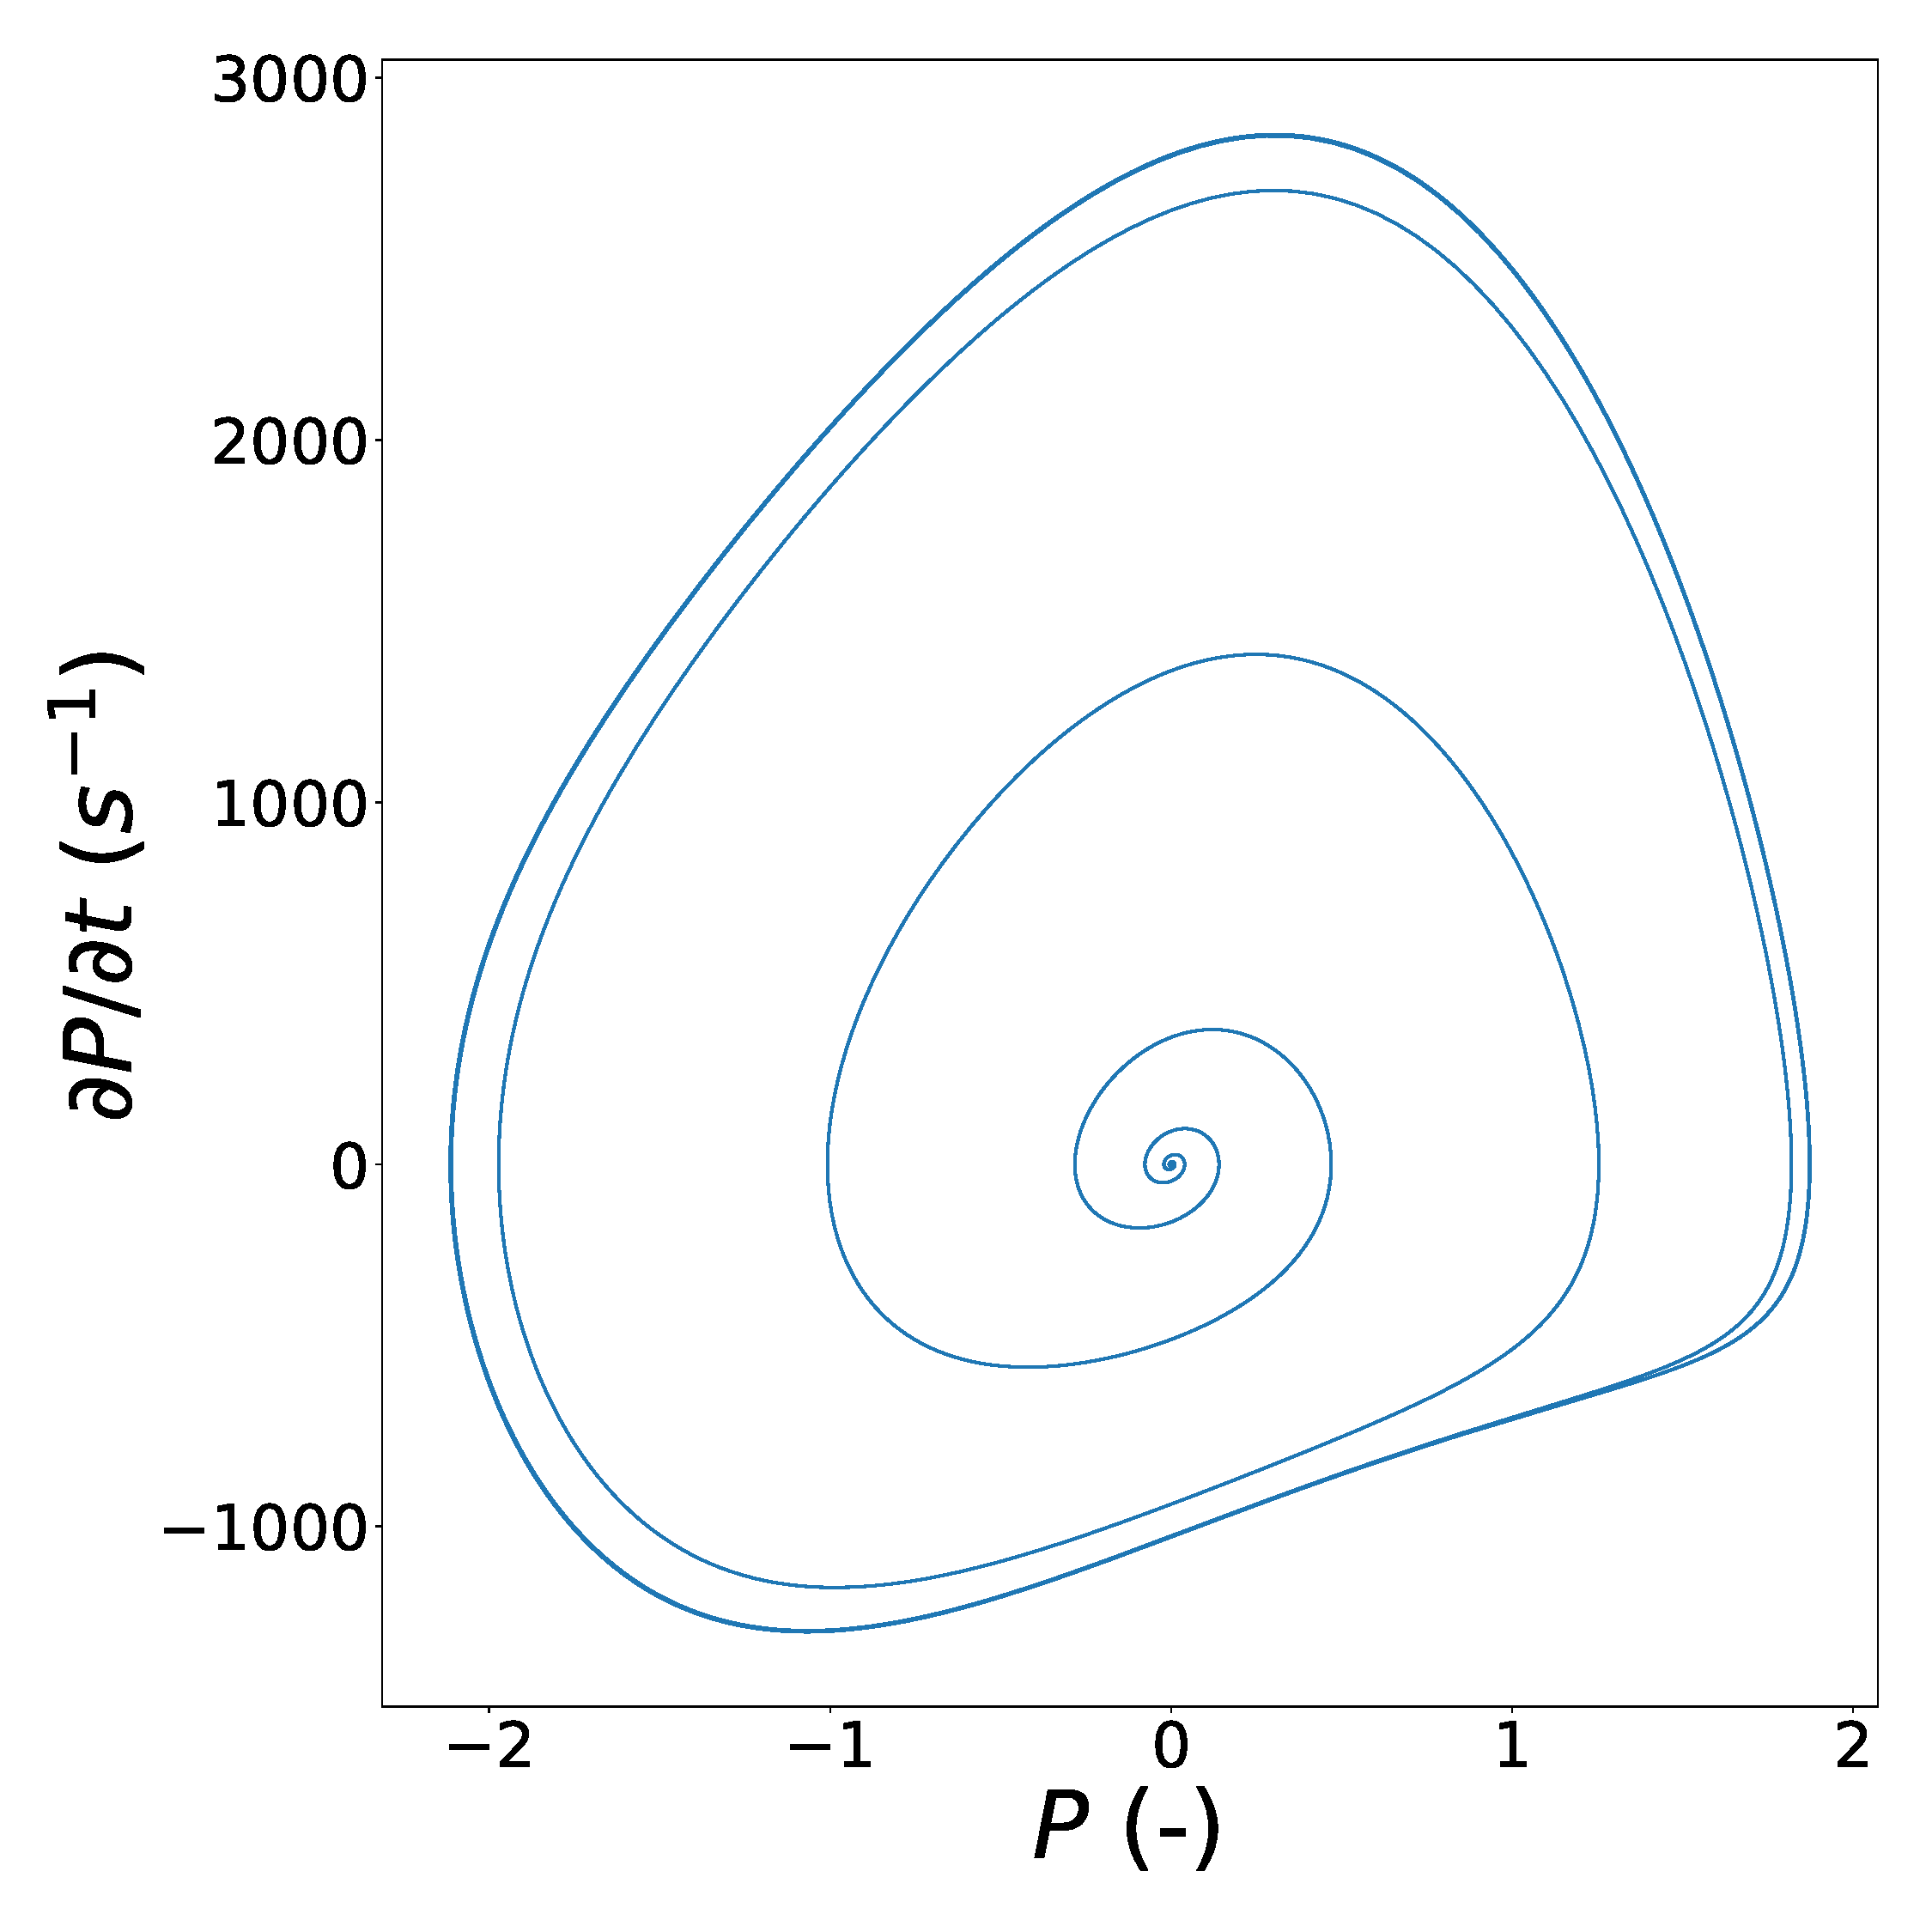
\includegraphics[width=\linewidth]{img/phase_diagram_N1.pdf}
        \caption{$N=1$}
        \label{fig:VDP_phase_N1}
    \end{subfigure}
    \hfill
    \begin{subfigure}[b]{.24\linewidth}
        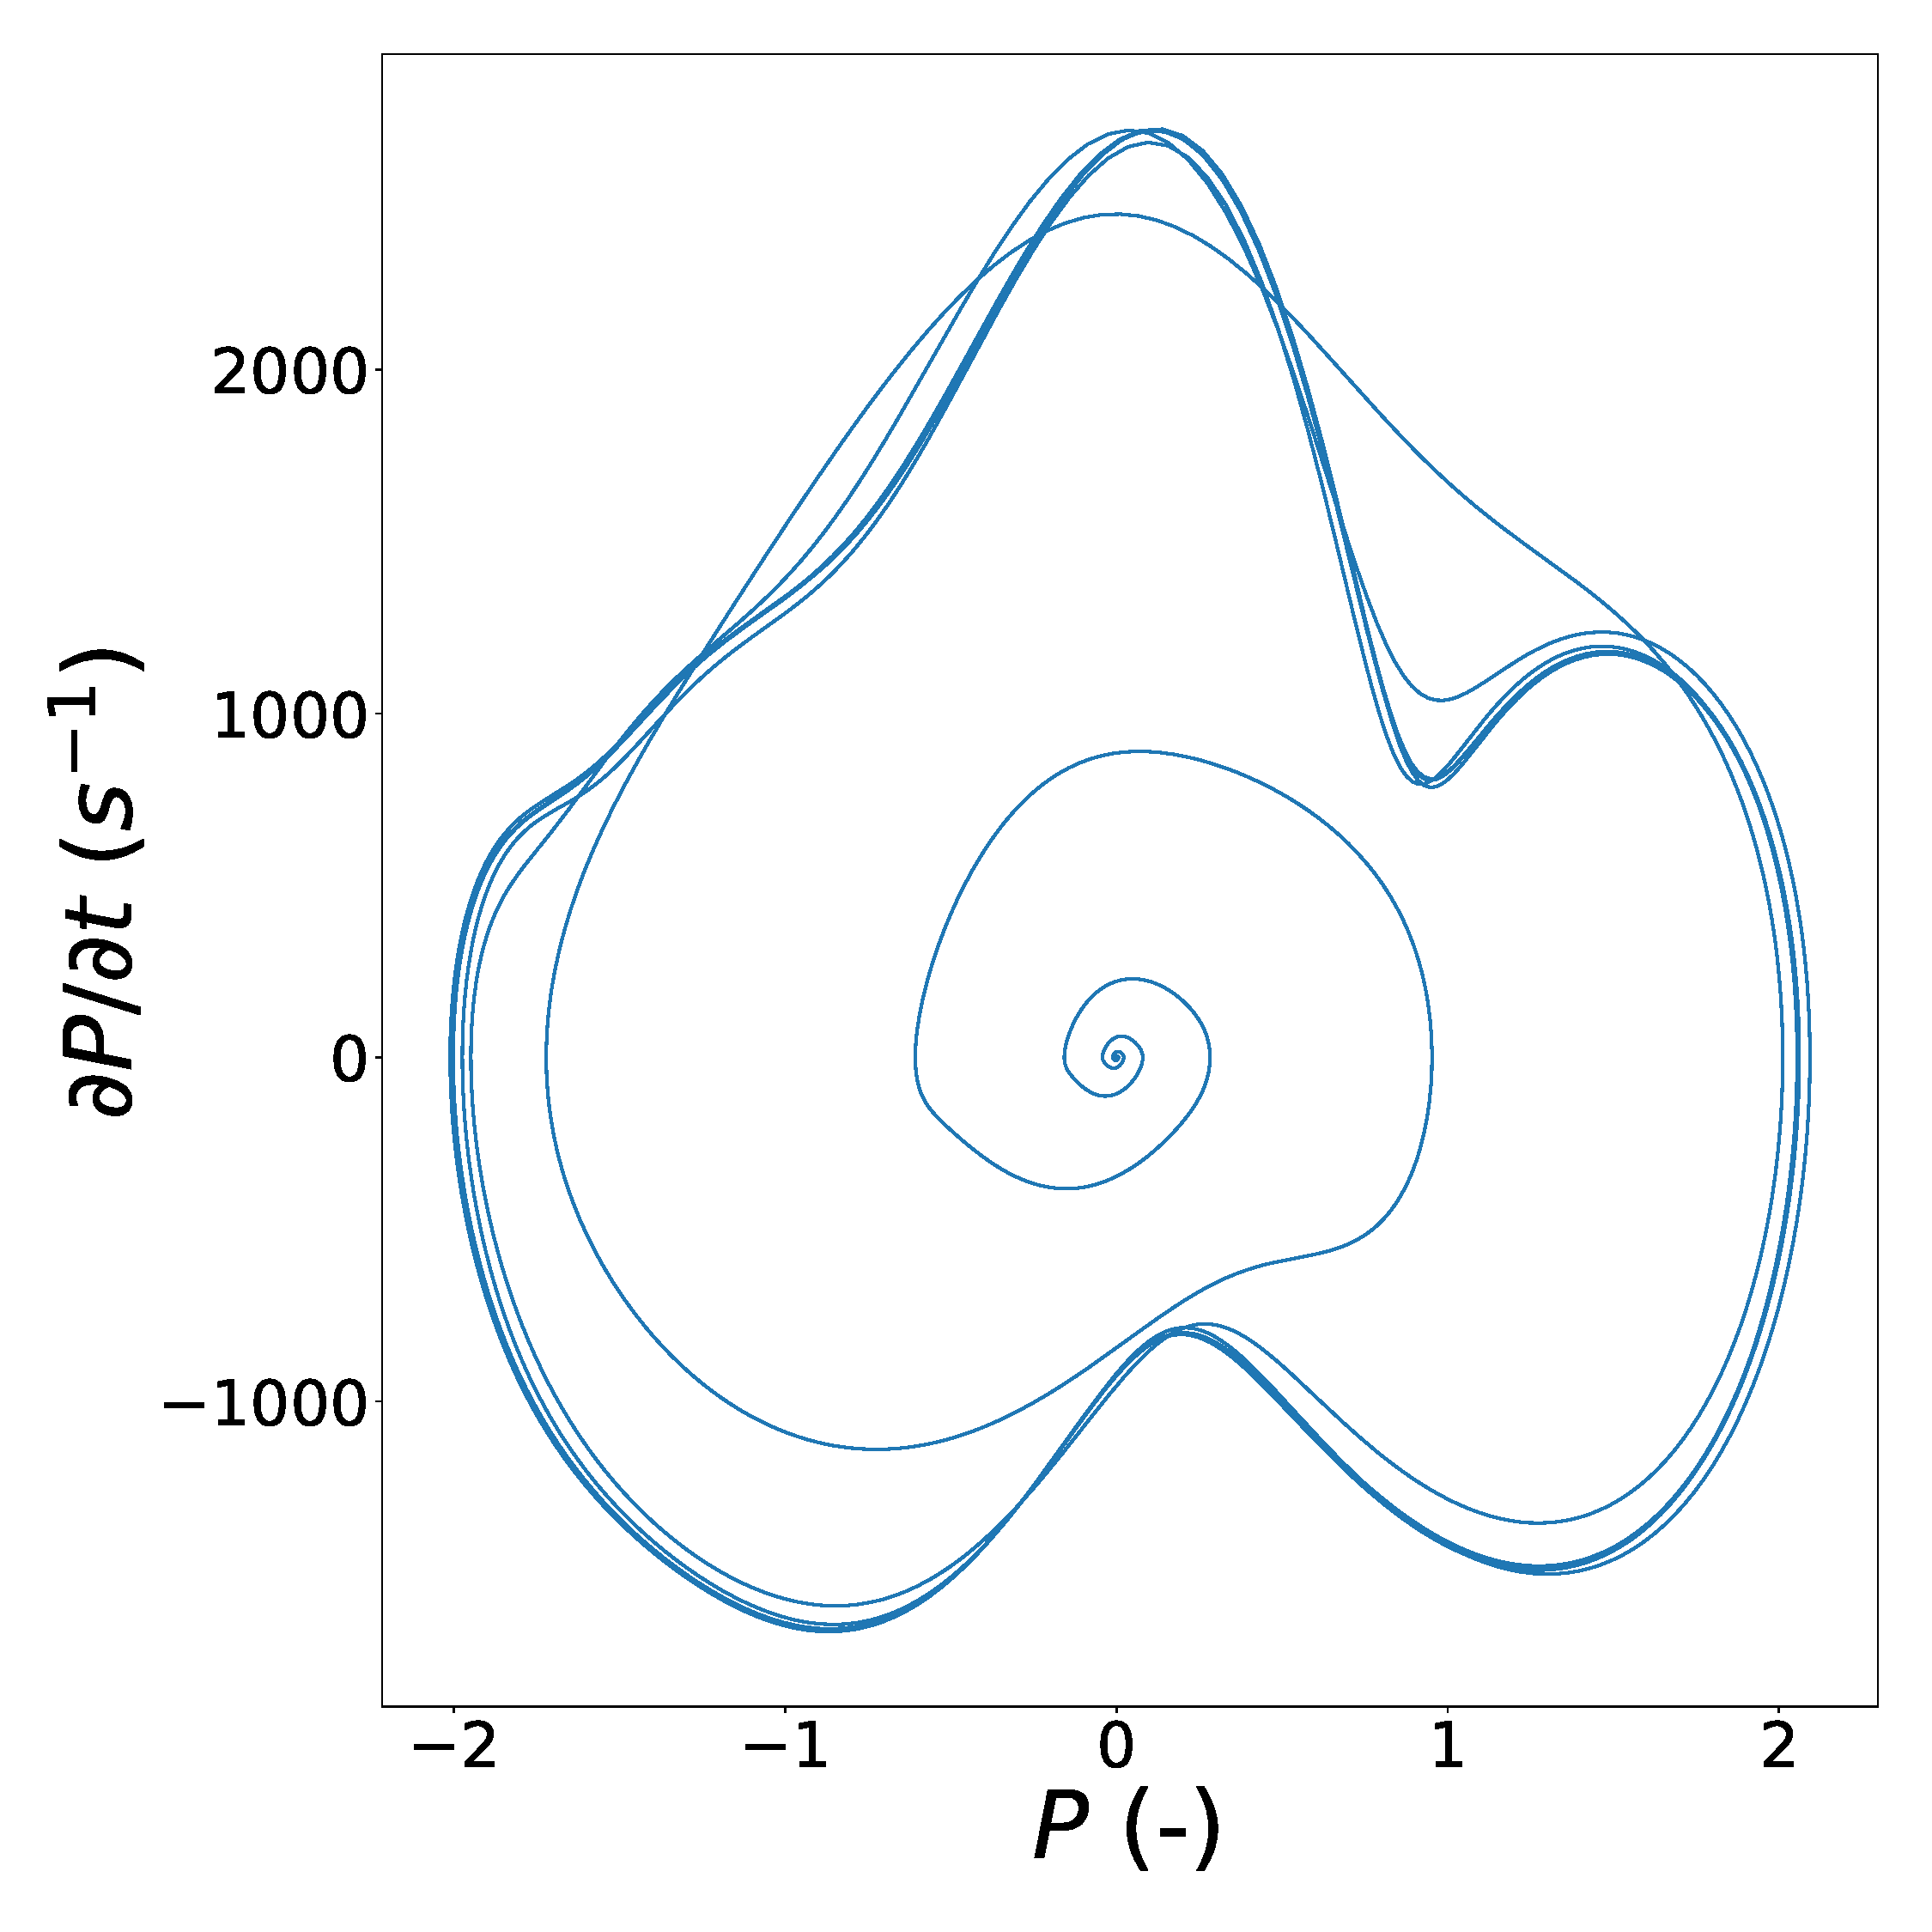
\includegraphics[width=\linewidth]{img/phase_diagram_N2.pdf}
        \caption{$N=2$}
        \label{fig:VDP_phase_N2}
    \end{subfigure}
    \hfill
    \begin{subfigure}[b]{.24\linewidth}
        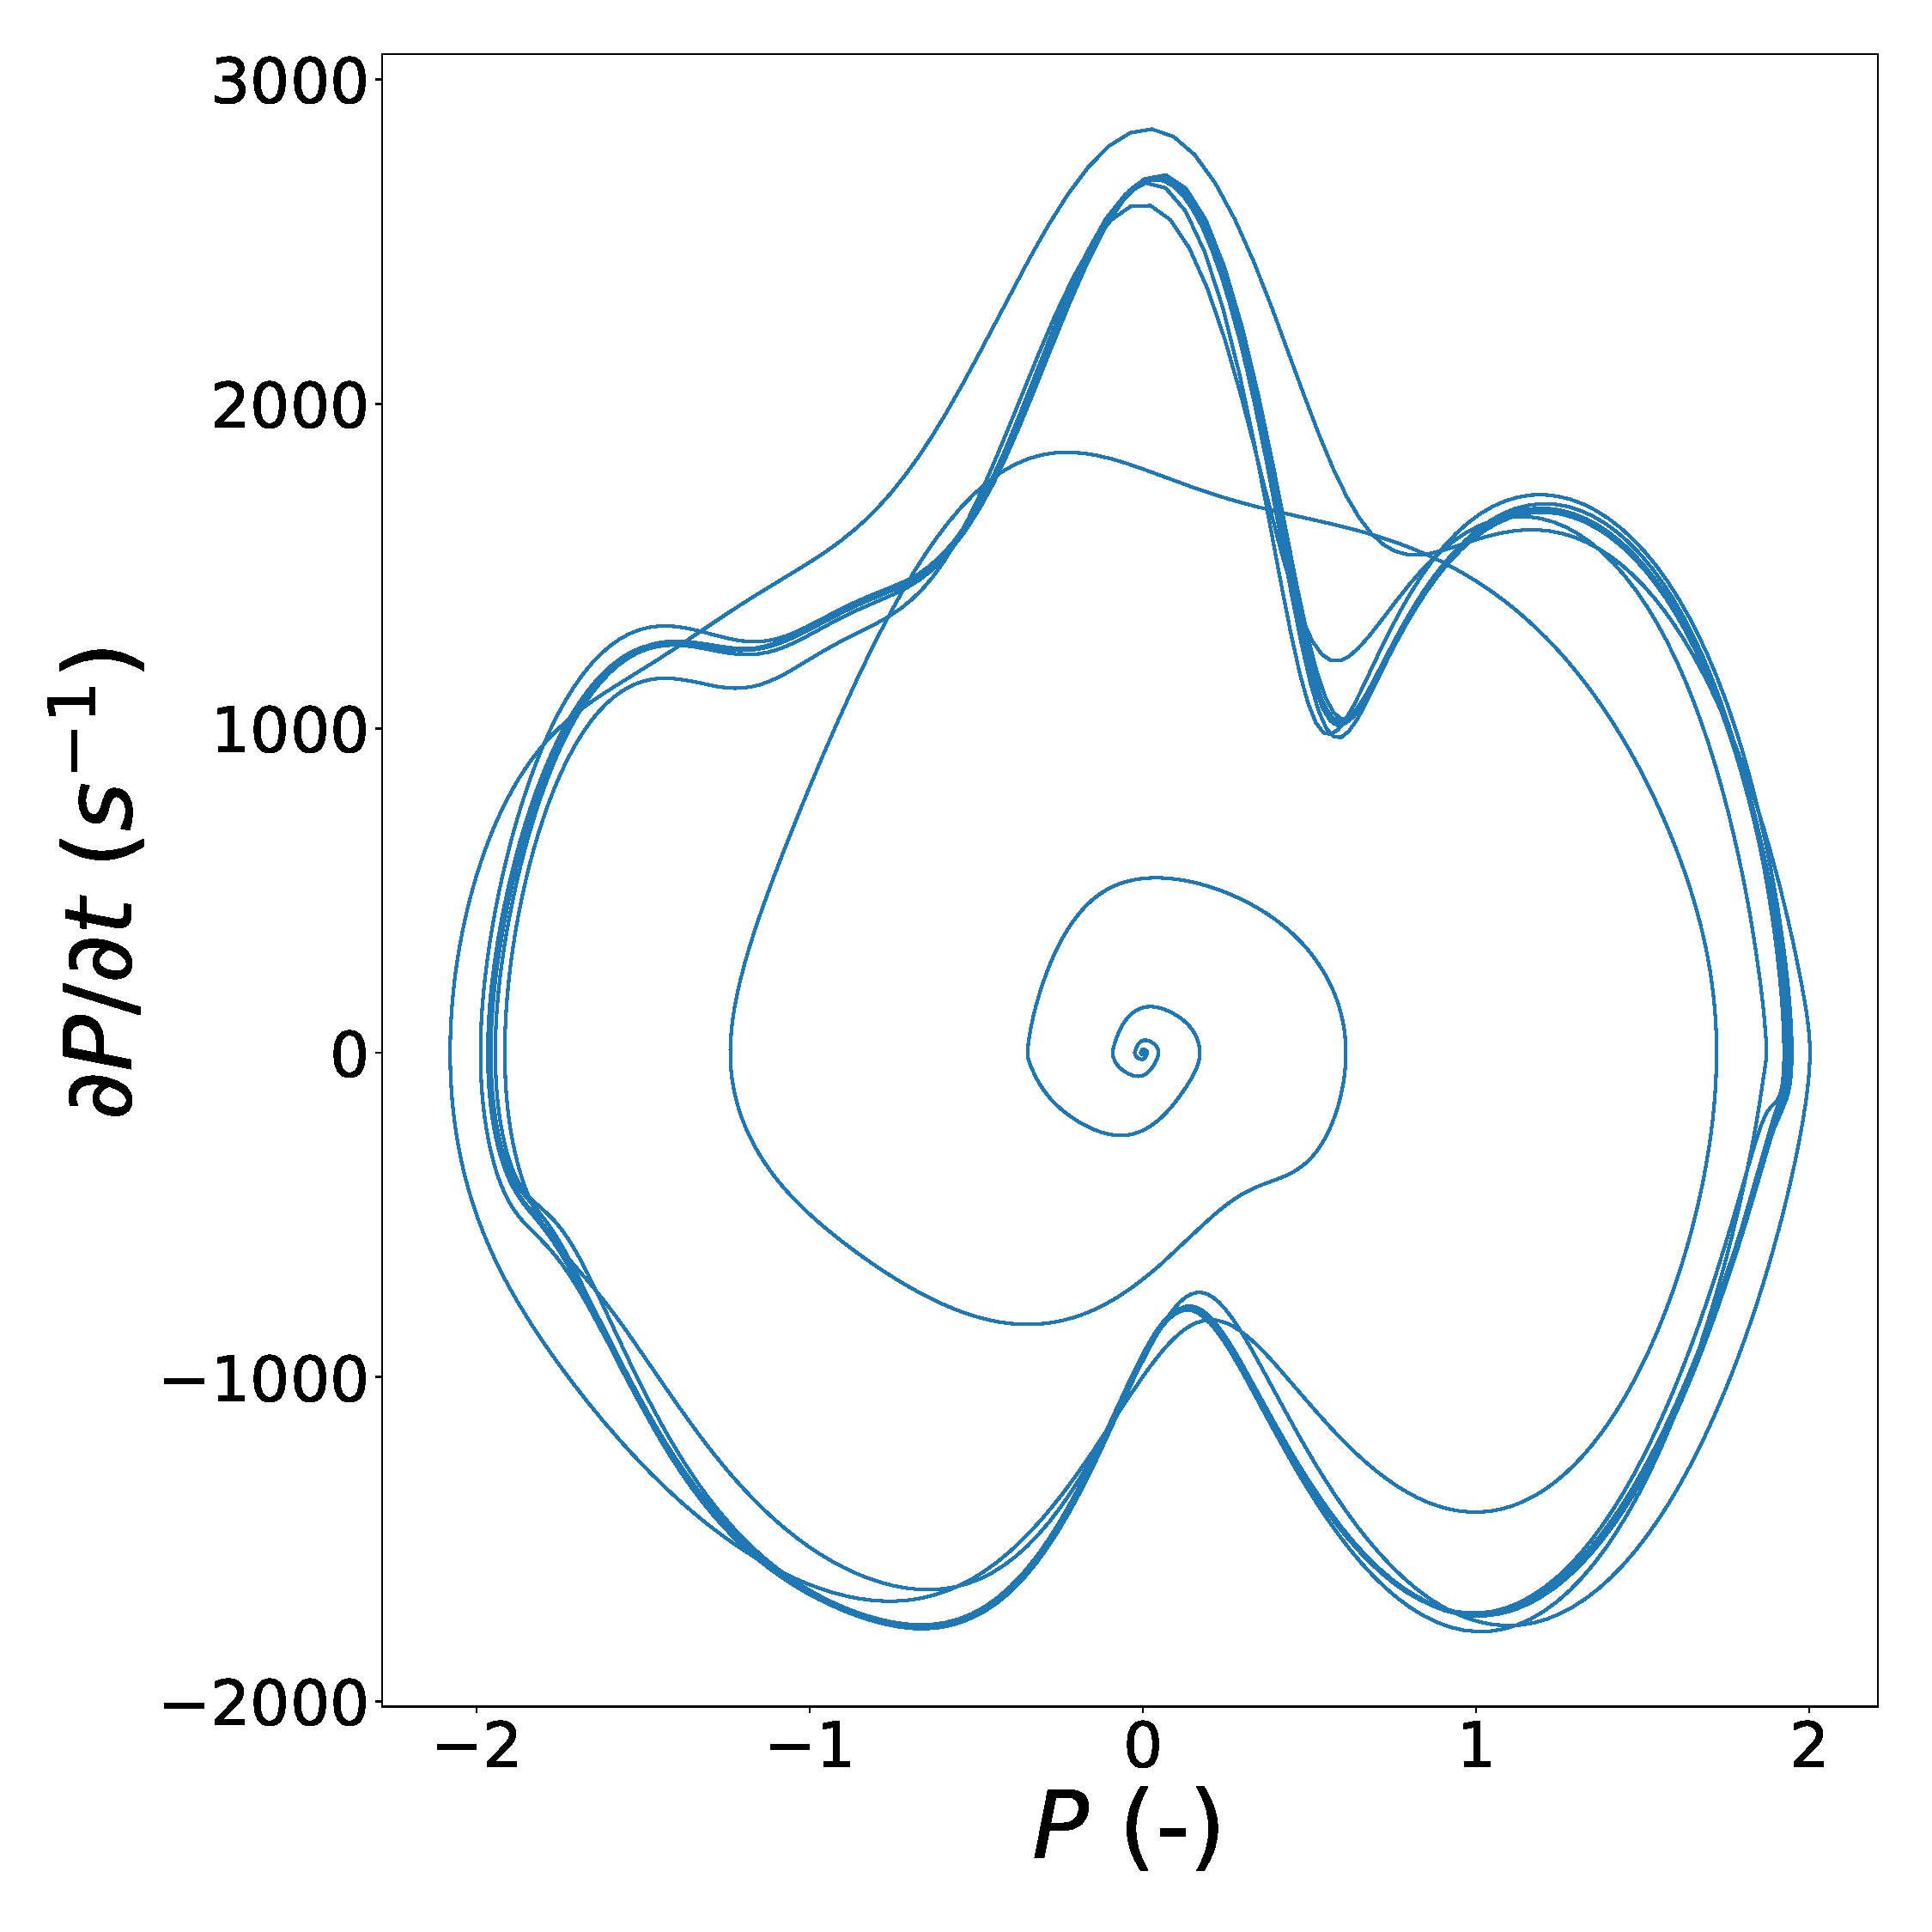
\includegraphics[width=\linewidth]{img/phase_diagram_N3.pdf}
        \caption{$N=3$}
        \label{fig:VDP_phase_N3}
    \end{subfigure}
    \hfill
    \begin{subfigure}[b]{.24\linewidth}
        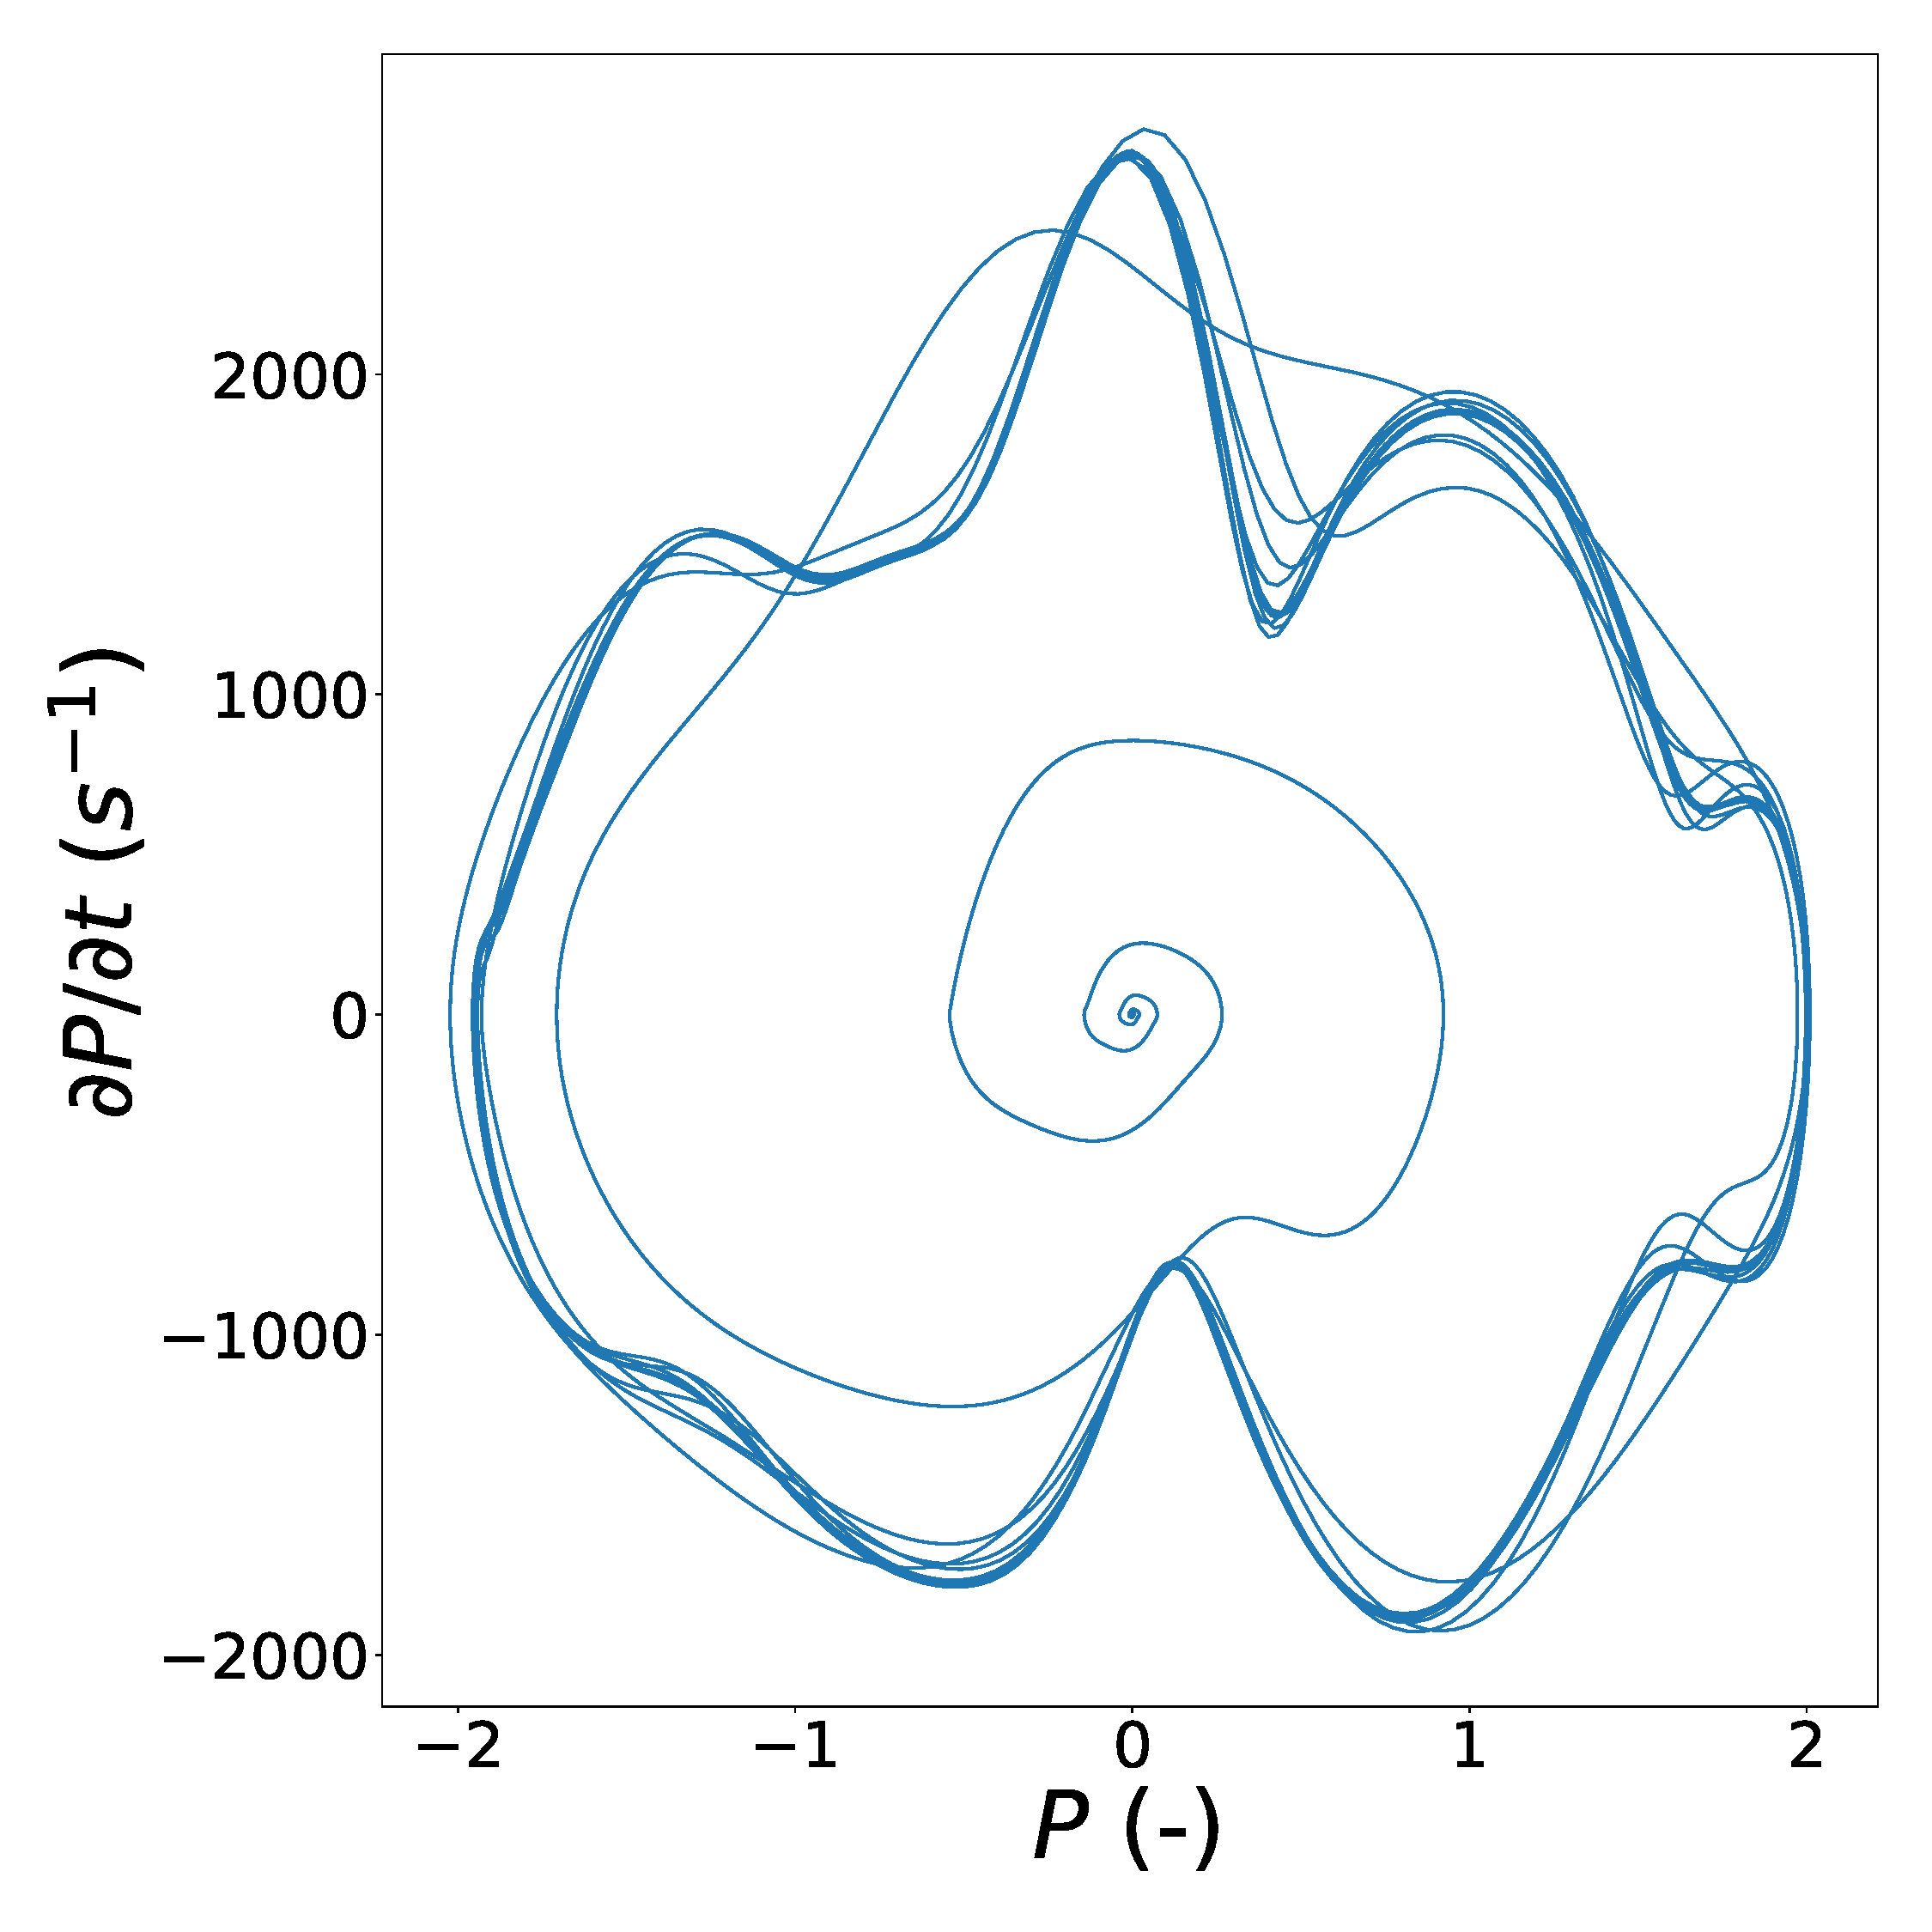
\includegraphics[width=\linewidth]{img/phase_diagram_N4.pdf}
        \caption{$N=4$}
        \label{fig:VDP_phase_N4}
    \end{subfigure}
    \caption{Evolution du flot $(P_0,\frac{\partial P_0}{\partial t})$ dans l'espace des phases durant l'attaque ($t<0.3$ s) pour $N$ modes. Le système est initialement perturbé par un saut de pression $P(t=0)=\epsilon$ ($\epsilon \ll 1$). Les solutions du système d'équations de Van der Pol convergent vers un cycle limite, dont la forme se complexifie avec N.}
    \label{fig:VDP_phase}
\end{figure}


\subsubsection{Cartes itérées}

\subsubsection{Guide d'onde}

Ligne à retard, complexification du modèle pour tenir compte des pertes plus importantes en hautes fréquences.